\documentclass[12pt,ngerman,parskip=half]{scrartcl}

\usepackage{babel}
\usepackage{tikz}
\usetikzlibrary{shapes}
% https://tikz.dev/tikz-arrows
\usetikzlibrary {arrows.meta} 
\usetikzlibrary {shadows} % für Schlagschatten 


\tikzset{punkt/.style = {
    shape=circle, fill = blue, minimum size = 0.25cm
}}

\tikzset{rechteck/.style = {
        shape  = rectangle, draw   = black,minimum height = 10cm,
        minimum width  = 14cm
}}

\tikzset{wolke/.style = {
shape=cloud, fill = red, minimum width=2cm,minimum height=2cm
}}

\tikzset{gwolke/.style = {wolke, fill = yellow}}

\usepackage{blindtext}

\begin{document}

\blindtext



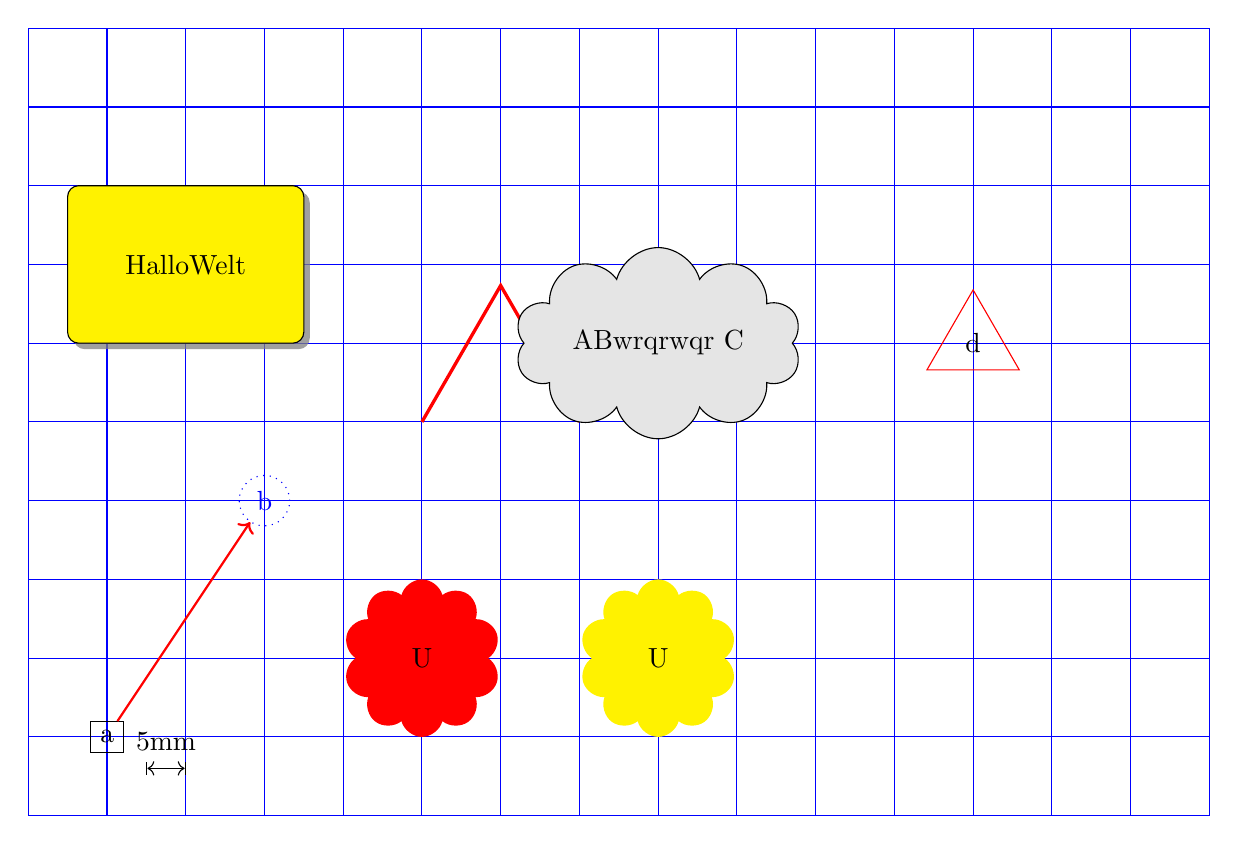
\begin{tikzpicture} 
\draw [step=1cm,blue,thin] (0,0) grid (15,10);
\draw[red,very thick] (5,5) -- ++(60:2)  -- ++(-60:2);

\node[rectangle,draw] (a) at (1,1){a};
\node[circle,draw,blue,dotted] (b) at (3,4){b};

\draw [->,red,thick] (a) -- (b);

\node[draw=red,regular polygon, regular polygon sides=3] (c) at (12,6){d};

\draw [|<->|] (1.5,.6) -- node[above=1mm] {5mm} (2,.6);

\node[cloud, draw, fill=gray!20, aspect=2] at (8,6) {ABwrqrwqr C};

\node[rectangle,draw,rounded corners,fill=yellow,minimum width=3cm,minimum height=2cm,drop shadow={opacity=0.75}] (a) at (2,7){HalloWelt};

\node[wolke] (e) at (5,2){U};

\node[gwolke] (d) at (8,2){U};

\end{tikzpicture}

\blindtext

\begin{tikzpicture}[node distance=3cm]
  \node (r) at (0,0) [rechteck] {};
  \node[label=r.center] at (r.center) [punkt] {};
  \node[label=r.north] at (r.north) [punkt] {};
  \node[label=r.south] at (r.south) [punkt] {};
  \node[label=r.east] at (r.east) [punkt] {};
  \node[label=r.west] at (r.west) [punkt] {};
  \node[label=r.north east] at (r.north east) [punkt] {};
  \node[label=r.north west] at (r.north west) [punkt] {};
  \node[label=r.south east] at (r.south east) [punkt] {};
  \node[label=r.south west] at (r.south west) [punkt] {};
\end{tikzpicture}



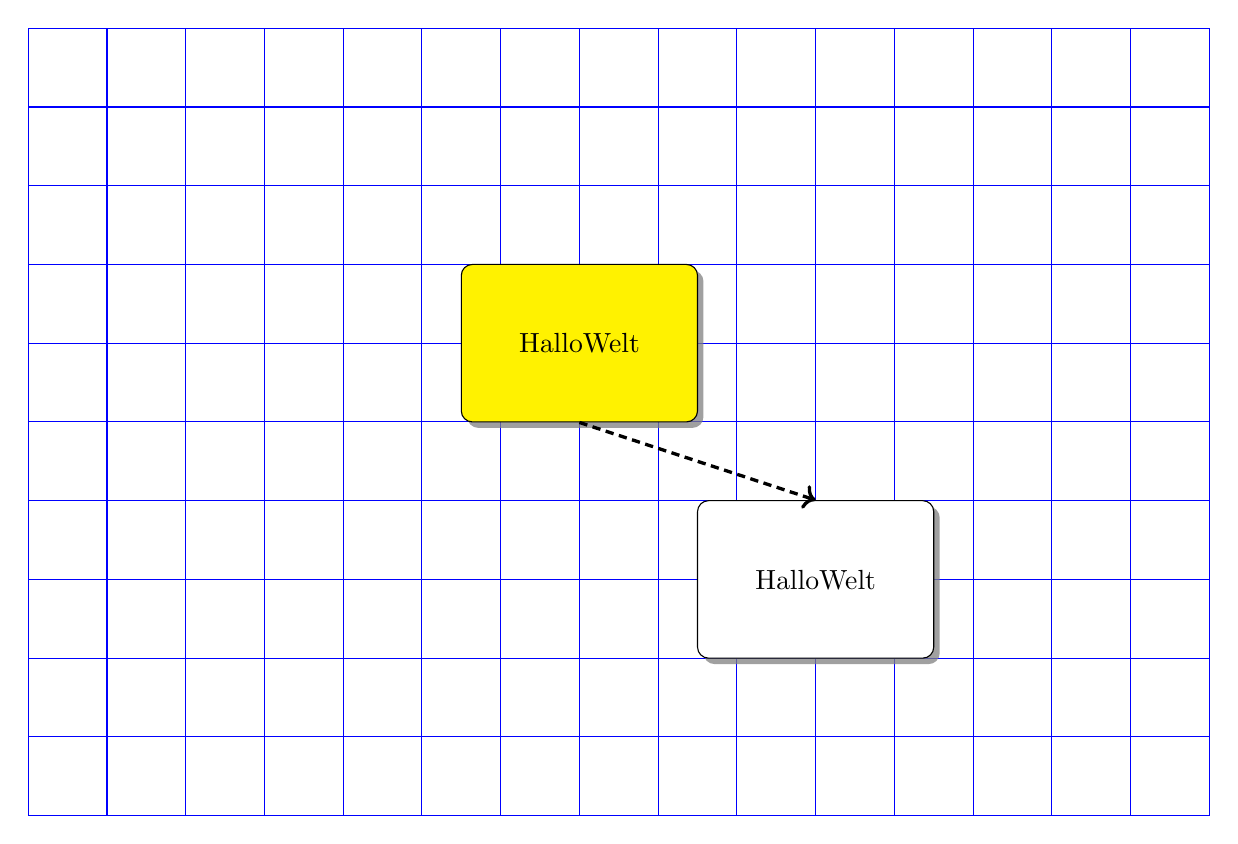
\begin{tikzpicture} 
\draw [step=1cm,blue,thin] (0,0) grid (15,10);

\node[rectangle,draw,rounded corners,fill=yellow,minimum width=3cm,minimum height=2cm,drop shadow={opacity=0.75}] (a) at (7,6){HalloWelt};

\node[rectangle,draw,rounded corners,fill=white,minimum width=3cm,minimum height=2cm,drop shadow={opacity=0.75}] (b) at (10,3){HalloWelt};

\draw[->,very thick, densely dashed](a.south) -- (b.north);

\end{tikzpicture}

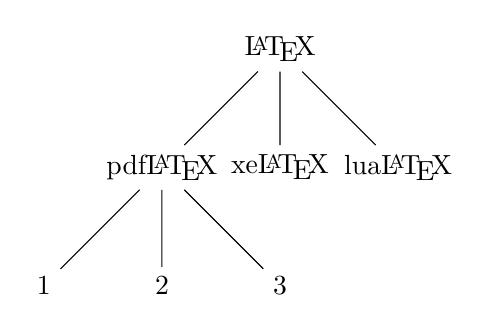
\begin{tikzpicture} 


\node{\LaTeX} 
child { node {pdf\LaTeX}
	child { node {1} } 
	child { node {2} }	
	child { node {3} }
}
child {node {xe\LaTeX} }
child {node {lua\LaTeX} }
;

\end{tikzpicture}




\end{document}